\chapter{Diagrams}
    \begin{figure}[H]
        \begin{center}
            % original from idea
            %\scalebox{0.34}[0.475]{\includegraphics{img/src/maven-deps-tree.pdf}}
            \scalebox{0.6}{\includegraphics{img/src/maven-deps-tree.pdf}}
            \caption{Dependency tree of maven artifacts.}
            \label{appen:maven-deps}
        \end{center}
    \end{figure}

    \begin{figure}[H]
        \begin{center}
            \scalebox{0.35}[0.21]{\includegraphics[angle=90]{img/src/class-diagram.pdf}}
            \caption{Partial class diagram of \texttt{datamining-forecast} and \texttt{datamining-api}.}
            \label{appen:class-diagram}
        \end{center}
    \end{figure}

\chapter{Predictive Charts}
    \begin{figure}[H]
        \begin{center}
            \scalebox{0.6}[0.443]{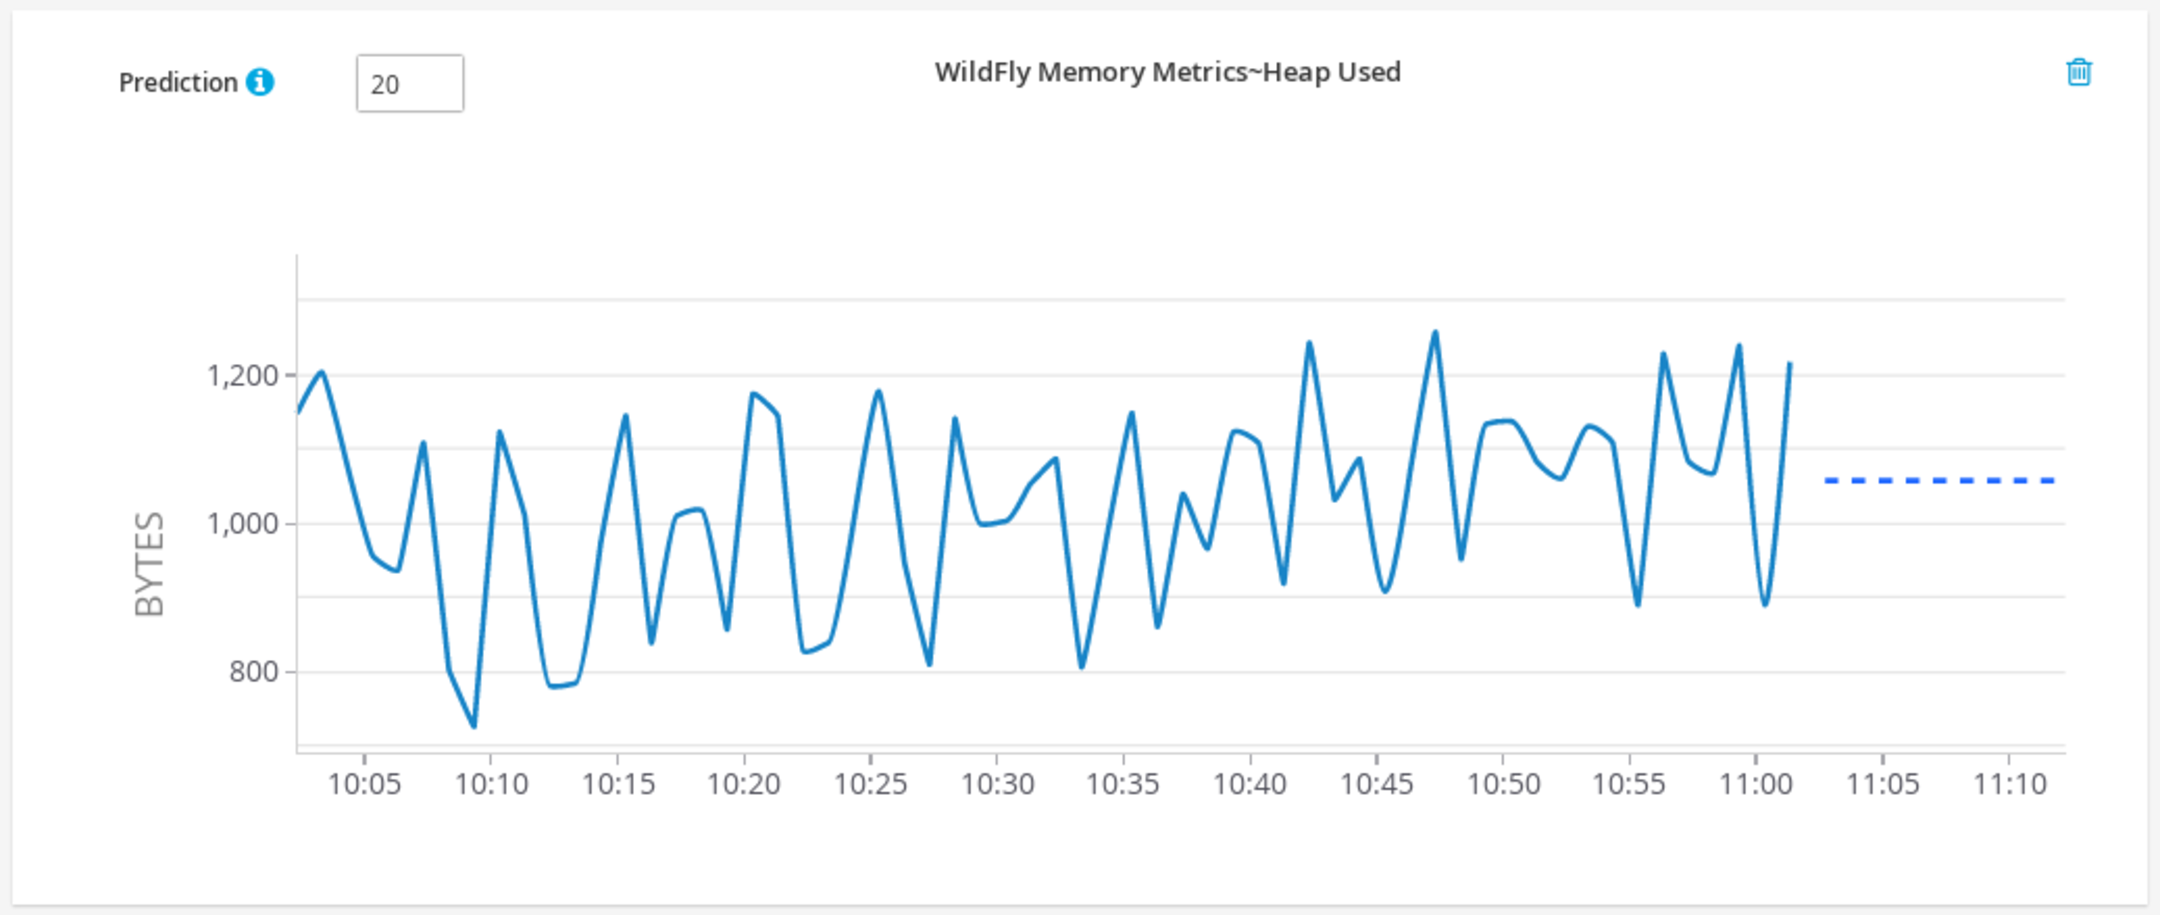
\includegraphics[angle=90]{img/hawkular-simple.pdf}}
            \caption{Predictive chart for simple exponential smoothing.}
            \label{appen:hawkular-simple}
        \end{center}
    \end{figure}
    \begin{figure}[H]
        \begin{center}
            \scalebox{0.6}[0.5]{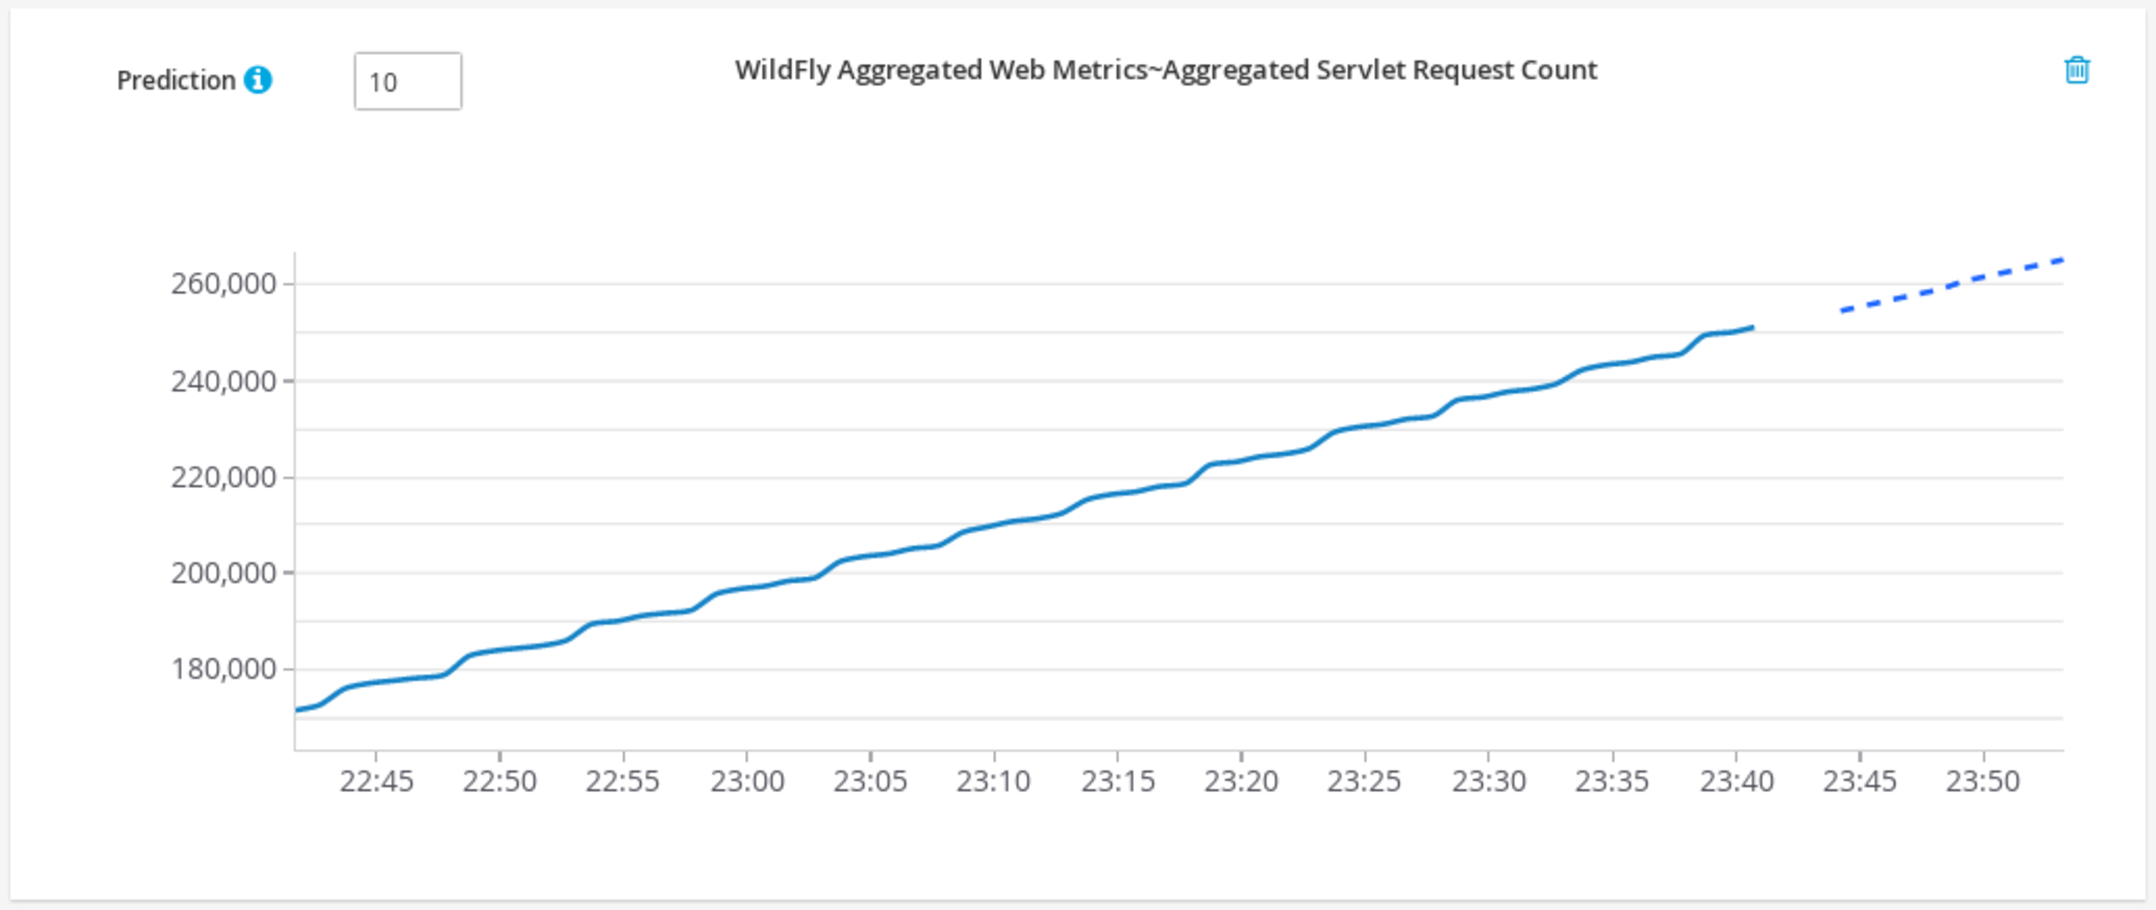
\includegraphics[angle=90]{img/hawkular-double.pdf}}
            \caption{Predictive chart for double exponential smoothing.}
            \label{appen:hawkular-double}
        \end{center}
    \end{figure}
    \begin{figure}[H]
        \begin{center}
            \scalebox{0.6}[0.5]{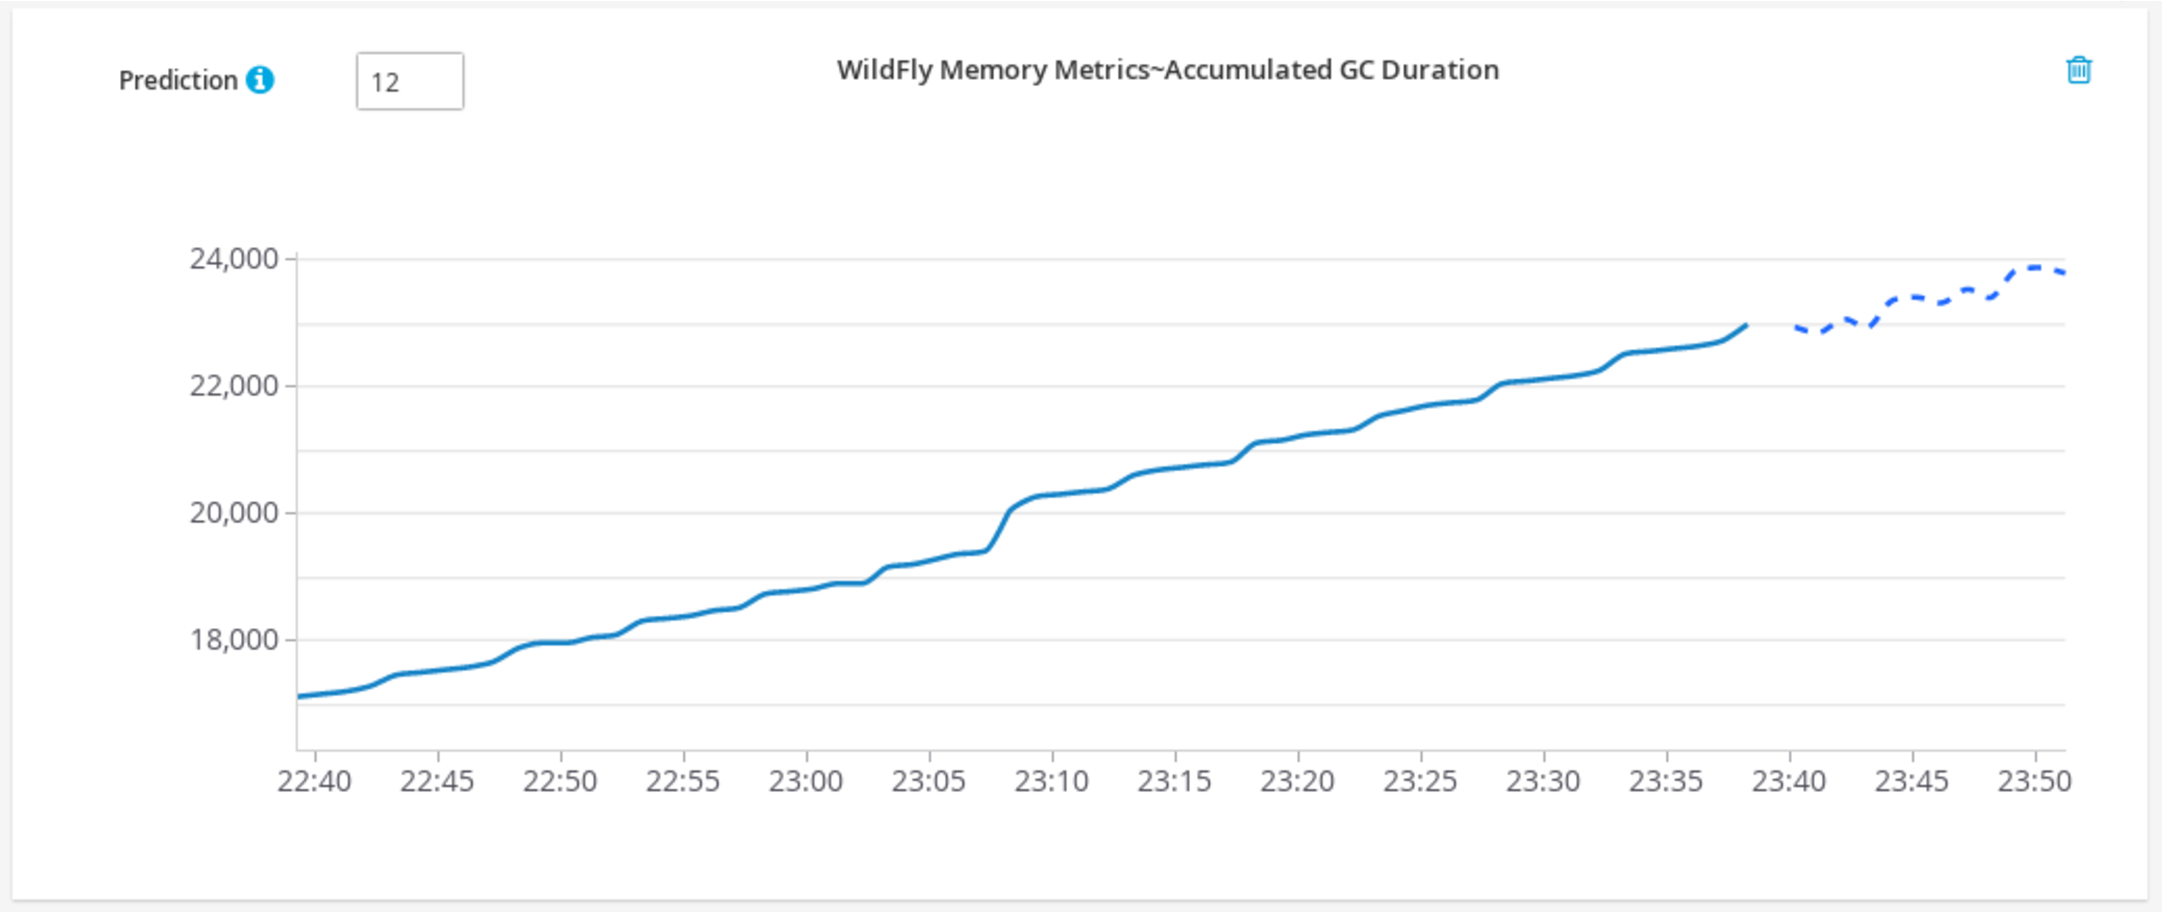
\includegraphics[angle=90]{img/hawkular-triple.pdf}}
            \caption{Predictive chart for triple exponential smoothing.}
            \label{appen:hawkular-triple}
        \end{center}
    \end{figure}

\chapter{Testing Time Series Samples} \label{appen:testing-samples}
    \begin{figure}[H]
        \begin{center}
            \scalebox{0.22}[0.62]{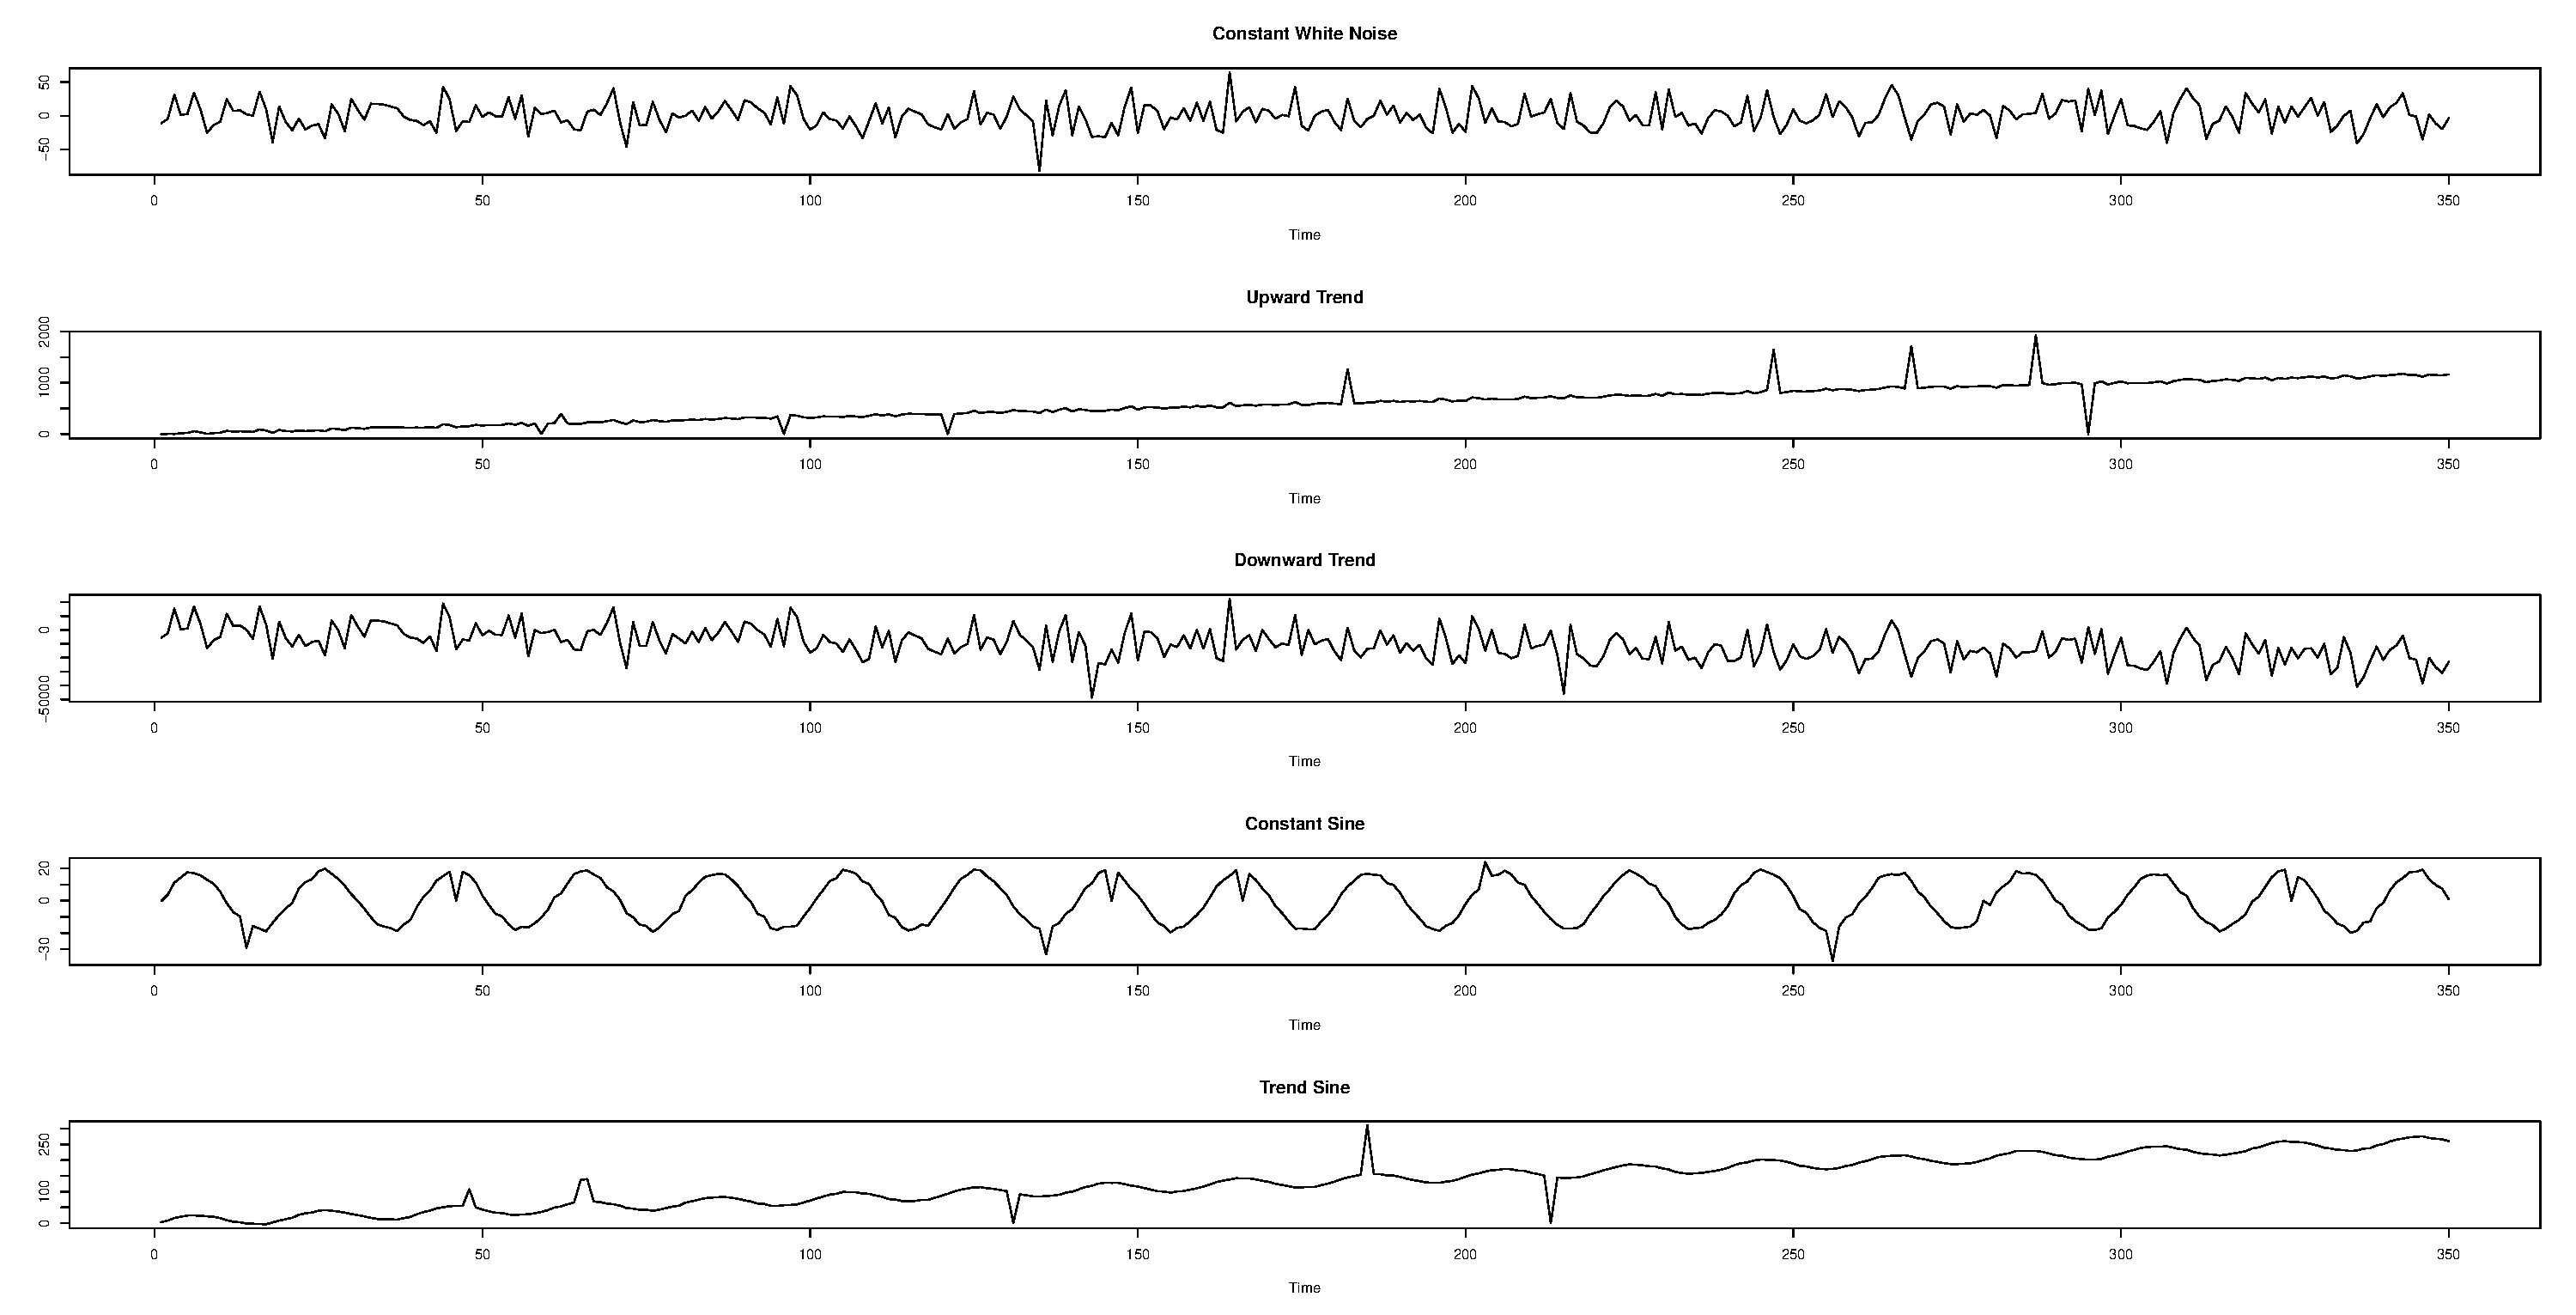
\includegraphics[angle=0]{img/testing-time-series.pdf}}
            \caption{Time series samples for evaluation.}
            \label{appen:img-testing-samples}
        \end{center}
    \end{figure}

\chapter{Tests Results} \label{appen:chap:results}

    \begin{table}[h]
        \begin{center}
            \begin{tabular}{c|c|c|c|c|c}
                \textbf{Test case} &
                \rotatebox{90}{wn} &  \rotatebox{90}{\texttt{trendUpLow}} & \rotatebox{90}{\texttt{trendDownHigh}} &
                \rotatebox{90}{\texttt{sine}} & \rotatebox{90}{\texttt{sineTrend}} \\ \hline \hline
                \multirow{2}{*}{48\,--\,12 (1)}   & 252.60 & 4293.10 & 59074630.35 & 19.91 & 291.89 \\
                                                  & 251.72 & 4602.83 & 57931198.55 & 19.97 & 291.90 \\ \hline
                \multirow{2}{*}{100\,--\,12 (1)}  & 247.72 & 702.52  & 117983966.67 & 23.54 & 25.82 \\
                                                  & 252.96 & 513.46 & 124329179.62 & 23.54 & 26.30 \\ \hline
                \multirow{2}{*}{200\,--\,12 (1)}  & 380.51 & 862.58 & 100868036.49 & 45.14 & 50.91 \\
                                                  & 380.57 & 718.39 & 101969913.50 & 45.14 & 47.95 \\ \hline \hline

                \multirow{2}{*}{48\,--\,12 (6)}   & 333.07 & 7071.66 & 90579713.93 & 483.70 & 1772.85\\
                                                  & 325.33 & 7206.03 & 89687108.81 & 483.88 & 1772.86 \\ \hline
                \multirow{2}{*}{100\,--\,12 (6)}  & 287.00 & 1916.31 & 125727085.38 & 420.33 & 346.06 \\
                                                  & 289.63 & 1531.48 & 130162180.73 & 420.33 & 347.18 \\ \hline
                \multirow{2}{*}{200\,--\,12 (6)}  & 325.67 & 1457.51 & 172882341.31 & 394.90 & 2734.56 \\
                                                  & 327.13 & 1132.87 & 172309610.96 & 394.90 & 2733.64 \\ \hline \hline

                \multirow{2}{*}{48\,--\,12 (12)}  & 271.78 & 7556.76 & 71166890.64 & 535.57 & 2956.52 \\
                                                  & 276.16 & 7742.00 & 71094737.26 & 535.46 & 2956.52 \\ \hline
                \multirow{2}{*}{100\,--\,12 (12)} & 239.68 & 12726.82 & 104525954.16 & 513.42 & 288.09 \\
                                                  & 251.44 & 12416.04 & 112937185.50 & 513.42 & 286.96 \\ \hline
                \multirow{2}{*}{200\,--\,12 (12)} & 381.57 & 2875.74 & 197649156.81 & 562.27 & 2064.04 \\
                                                  & 381.71 & 2316.18 & 196658315.76 & 562.27 & 2077.42 \\ \hline
            \end{tabular}
            \caption{Test results in MSE for simple exponential smoothing.}
            \label{appen:tab:simple-results}
        \end{center}
    \end{table}

    \begin{table}[h]
        \begin{center}
            \begin{tabular}{c|c|c|c|c|c}
                \textbf{Test case}  & \rotatebox{90}{wn} &
                \rotatebox{90}{\texttt{trendUpLow}} & \rotatebox{90}{\texttt{trendDownHigh}} &
                \rotatebox{90}{\texttt{sine}} & \rotatebox{90}{\texttt{sineTrend}} \\ \hline \hline
                \multirow{2}{*}{48\,--\,12 (1)}   & 272.33 & 3617.53 & 65694458.22 & 22.70 & 668.61 \\
                                                  & 279.60 & 3574.63 & 66644587.71 & 20.41 & 659.66 \\ \hline
                \multirow{2}{*}{100\,--\,12 (1)}  & 282.50 & 190.63 & 90967195.65 & 8.46 & 26.17 \\
                                                  & 302.91 & 193.77 & 93267732.29 & 9.40 & 25.61 \\ \hline
                \multirow{2}{*}{200\,--\,12 (1)}  & 399.27 & 361.50 & 108286781.11 & 35.56 & 48.96 \\
                                                  & 405.67 & 347.69 & 109496254.07 & 38.48 & 48.21 \\ \hline \hline

                \multirow{2}{*}{48\,--\,12 (6)}   & 354.67 & 6324.32 & 86541840.59 & 880.76 & 8031.60 \\
                                                  & 320.00 & 6454.35 & 77856708.99 & 856.96 & 7843.41 \\ \hline
                \multirow{2}{*}{100\,--\,12 (6)}  & 323.09 & 263.81 & 110815056.99 & 636.99 & 449.11 \\
                                                  & 332.08 & 253.23 & 100878861.50 & 673.94 & 420.09 \\ \hline
                \multirow{2}{*}{200\,--\,12 (6)}  & 324.50 & 316.76 & 167489984.23 & 811.24 & 2958.53 \\
                                                  & 340.14 & 374.38 & 162368879.38 & 830.81 & 2933.63 \\ \hline \hline

                \multirow{2}{*}{48\,--\,12 (12)}  & 275.92 & 3077.24 & 65058787.15 & 4394.80 & 29063.69 \\
                                                  & 299.00 & 3068.45 & 72999868.22 & 3921.33 & 28324.64 \\ \hline
                \multirow{2}{*}{100\,--\,12 (12)} & 272.97 & 13143.67 & 58829949.01 & 4919.03 & 565.68 \\
                                                  & 315.49 & 13449.97 & 76982996.39 & 4646.99 & 490.45 \\ \hline
                \multirow{2}{*}{200\,--\,12 (12)} & 376.87 & 423.64 & 186182717.66 & 5777.67 & 2507.91 \\
                                                  & 381.13 & 499.08 & 173511817.12 & 5462.19 & 2489.15 \\ \hline
            \end{tabular}
            \caption{Test results in MSE for double exponential smoothing.}
            \label{appen:tab:double-results}
        \end{center}
    \end{table}

    \begin{table}[h]
        \begin{center}
            \begin{tabular}{c|c|c}
                \textbf{Test case} &
                \rotatebox{90}{\texttt{sine}} & \rotatebox{90}{\texttt{sineTrend}} \\ \hline \hline
                \multirow{2}{*}{48\,--\,12 (1)}   & 11.24 & 25.08 \\
                                                  & 8.07 & 20.15 \\ \hline
                \multirow{2}{*}{100\,--\,12 (1)}  & 2.29 & 43.64   \\
                                                  & 2.09 & 57.07 \\ \hline
                \multirow{2}{*}{200\,--\,12 (1)}  & 15.92 & 88.18 \\
                                                  & 15.74 & 73.84 \\ \hline \hline

                \multirow{2}{*}{48\,--\,12 (6)}   & 9.26 & 390.64 \\
                                                  & 4.07 & 693.93 \\ \hline
                \multirow{2}{*}{100\,--\,12 (6)}  & 3.09 & 34.05 \\
                                                  & 2.44 & 37.11 \\ \hline
                \multirow{2}{*}{200\,--\,12 (6)}  & 4.19 & 1853.59 \\
                                                  & 5.65 & 1908.62 \\ \hline \hline

                \multirow{2}{*}{48\,--\,12 (12)}  & 4.31 & 965.75 \\
                                                  & 4.07 & 693.93 \\ \hline
                \multirow{2}{*}{100\,--\,12 (12)} & 2.26 & 8.44 \\
                                                  & 2.15 & 7.48 \\ \hline
                \multirow{2}{*}{200\,--\,12 (12)} & 0.95 & 1954.75 \\
                                                  & 2.63 & 1924.38 \\ \hline
            \end{tabular}
            \caption{Test results in MSE for triple exponential smoothing.}
            \label{appen:tab:triple-results}
        \end{center}
    \end{table}

\chapter{Source Code Metrics}
    \paragraph*{Number of Java files:} 105
    \paragraph*{Number of lines:} 9782
    \paragraph*{Size of the WAR archive of \texttt{hawkular-dataminig-dist} module} : 8744B

\chapter{Content of the Attachment}
    \paragraph*{Directory \texttt{doc}:} \LaTeX source code of this thesis.
    \paragraph*{Directory \texttt{src}:} source code of Data Mining module.
    \paragraph*{Directory \texttt{src-hawkular}:} source code of Hawkular with integrated Data Mining.
    \paragraph*{Directory \texttt{bin}:} binaries of Data Mining and Hawkular with integrated Data Mining.
